%!TEX root = main.tex
\chapter*{Vorbemerkungen}

\section*{Quellen}

Viele der rein mathematischen Bemerkungen, Aussagen und Beispiele sind Abgeleitet aus \cite{merziger2024repetitorium} und \cite{gollmann2017mathematik}. Im Literaturverzeichnis finden sich Selbstverständlich andere zitierte Arbeiten.

\section*{Errata}

Bezüglich etwaigen Fehlern bitte einen \emph{issue} auf github zu eröffnen: \href{https://github.com/hrtlacek/matheFuerTonmeisterinnen/issues}{hier}. Größere Kommentare, Zweifel an Richtigkeit, Feedback etc, sehr gerne auch direkt per mail: \texttt{ptrk.lechner@gmail.com}.

Sehr gerne können Fehler, Korrekturen und Ergänzungen auch selbst geändert werden und ein \emph{pull request} gemacht werden.

\section*{Soundbeispiele}

Soundbeispiele sind in der Programmiersprache \texttt{FAUST} erstellt. Durch click auf das Lautsprecher Symbol sollte sich ein Browser öffnen in dem der entsprechende Klang in Echtzeit berechnet wird. Manche der Beispiele bieten Interaktionsmöglichkeit durch diverse Slider etc. Hier ein Beispiel:

\faust{Sinus, 150 Hz}{https://faustide.grame.fr/?autorun=1&voices=0&name=example&inline=aW1wb3J0KCJzdGRmYXVzdC5saWIiKTsKYW1wID0gaHNsaWRlcigiQW1wbGl0dWRlIiwgMC4yNSwgMCwgMSwgMC4wMDEpOnNpLnNtb287CnByb2Nlc3MgPSAob3Mub3NjKDE1MCkgKiBhbXApIDw6XyxfOw\%3D\%3D}

\emph{Zum Teil scheint es notwendig zu sein noch auf der großen 'RUN' Button links oben zu clicken.}

\begin{figure}[h!]
	\centering
	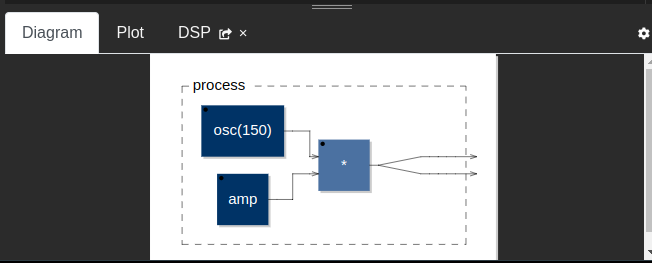
\includegraphics[width=0.8 \textwidth]{img/faust_diag.png}
	\caption{Block Diagramm in \texttt{FAUST}}
	\label{fig:faustBlock}
\end{figure}

Geneigten LeserInnen sei besonders empfohlen auch auf den 'Diagramm' button zu clicken um ein Blockdiagramm zu sehen dass dem Code/dem jeweiligen Konzept Entspricht.

Es kann nicht garantiert werden dass dieses Online service ständig online ist und die Details der Programmiersprache \texttt{FAUST} sind \textbf{nicht} Teil des Kurses.


\section*{Contributors}
Hier finden sich hoffentlich bald Menschen die diesen Text gelesen haben und Verbesserungsvorschläge gemacht haben.

% \section*{General TODOs}
% \begin{itemize}
% 	% \item indexing
% 	\item proof reading..
% 	% \item Page numbers
% 	% \item scheinbar wird derzeit teilweise Text 'verschluckt'. zb linearfaktorzerlegung.
% \end{itemize}
